\documentclass[12pt,a4paper,english,twoside,openany]{book}
\usepackage[german,english]{babel}
\usepackage[T1]{fontenc} 
\usepackage[latin1]{inputenc}
\usepackage{amsfonts}
\usepackage{amsmath}
\usepackage{latexsym}
\usepackage{amssymb}
\usepackage{epsfig}
\usepackage{moreverb}
\usepackage{rotating}
\usepackage{enumerate}
\usepackage{graphics, graphicx,wrapfig,lipsum}
\usepackage{fancybox}
\usepackage{picinpar,varioref,floatflt}
\usepackage{ae}
\usepackage{longtable}
\usepackage{textcomp}
\usepackage{float}
\usepackage{unizhdt}
\usepackage{adjustbox}
\usepackage{tocbibind}
\usepackage[hyphens]{url}
\usepackage[font=scriptsize]{caption}
\usepackage{hyperref}
\usepackage{listings}
\usepackage{dirtytalk}
\usepackage[section]{placeins}

\hypersetup{
    colorlinks,
    citecolor=black,
    filecolor=black,
    linkcolor=black,
    urlcolor=black
}
% \usepackage[
% backend=biber,
% style=alphabetic,
% sorting=ynt
% ]{biblatex}

%%%%%%%%%%%%%%%%%%%%%%%%%%%%%%%%%%%%%%%%%%%%%%%%%%

% Define the language of the diploma thesis
\selectlanguage{english}
%\selectlanguage{german}

%set bib file for citing
% \addbibresource{}

\pagestyle{headings}

\begin{document}

%%%%%%%%%%%%%%%%%%%%%%%%%%%%%%%%%%%%%%%%%%%%%%%%%%

% Define the author printed on the cover page
\author{Danijel Dordevic}
% Define the city and country of the author
\authorcity{Zurich, Switzerland}
% Define the student ID (Matrikelnummer)
%\studentid{15-709-116 }

% Define the title with optional subtitle
\title{Design and Development of a React-Native Supply Chain Tracking Application}
% Define the supervisors
\supervisors{Sina Rafati Niya, Prof. Burkhard Stiller}
% Define the submission date
\submissiondate{July 1, 2019}

%%%%%%%%%%%%%%%%%%%%%%%%%%%%%%%%%%%%%%%%%%%%%%%%%%

% Make the title page
\maketitle

% Make the imprint on the back of the cover page
\makeimprint

\pagenumbering{roman}

% Include the files of the diploma thesis
%\cleardoublepage
\chapter*{Abstract}
\addcontentsline{toc}{chapter}{Abstract}

\selectlanguage{english}

While traditional supply chain (SC) systems met their requirements, they eventually reached their limits especially in a sense they do not provide enough transparency for the final consumers. They are also highly specialized in supplying just specific goods, meaning they are not generic enough to be reused for other types of goods. This is especially true for food, which safety and transparency are paramount to the final consumers. Traditional SC systems require a lot of manual work which leaves room for errors and manipulating with goods. Also, traditional systems lack integration between different systems in the supply chain which requires more work in order to make those systems work together. The commence of the Internet changed the way how traditional SC systems functioned. The more agile and dynamic way of working was introduced. That allowed the consumers to interact with their products at any of its stages. While the traditional SC systems have been improved over the course of time, there is room to advance the existing SC systems to the next level, especially when speaking about the transparency and making them more user-friendly for the final consumers. In this independent study, the aforementioned requirements are addressed by developing the application that can be used by both consumers and producers. 




\selectlanguage{english}

\chapter*{Acknowledgments}
\addcontentsline{toc}{chapter}{Acknowledgments}

I would like to take the opportunity and thank my supervisors Sina Rafati, Prof. Dr. Burkhard Stiller, and other members of the Communication Systems Group at the University of Zurich for allowing me to pursue this Independent Study.

%\cleardoublepage


\tableofcontents

\cleardoublepage
\pagenumbering{arabic}
\chapter{Introduction}


\section{Motivation}


\section{Description of Work}


\section{Thesis Outline}



\chapter{Design and Implementation}

In this section the architectural decisions and implementation will be explain in details. The first part describes the overall architecture, system design, high level overview. Later, the back-end system will be explained that this application relies on. Lastly, the application itself will be explained in details starting from the technologies/frameworks used.

\section{System Design}


System design is the process of defining the elements of a system with all its components, modules and interfaces. It can take a bottom-up or top-down approach \cite{system_design_def}. A system diagram is a high-level diagram that depicts the boundaries between the system and its environment. The figure \ref{fig:system_diagram} shows the high-level overview of the components and actors within the system. It can be seen that the mobile application plays the central role. It is a mediator between the producers and consumers, and the back-end system. It shows that the producers can generate qr codes, store the data on the back-end system, and that the consumers can later validate products by scanning the products/qr codes. This means that this application can be used both by consumers and producers which will be explained in details in the following section.

\begin{figure}[ht]
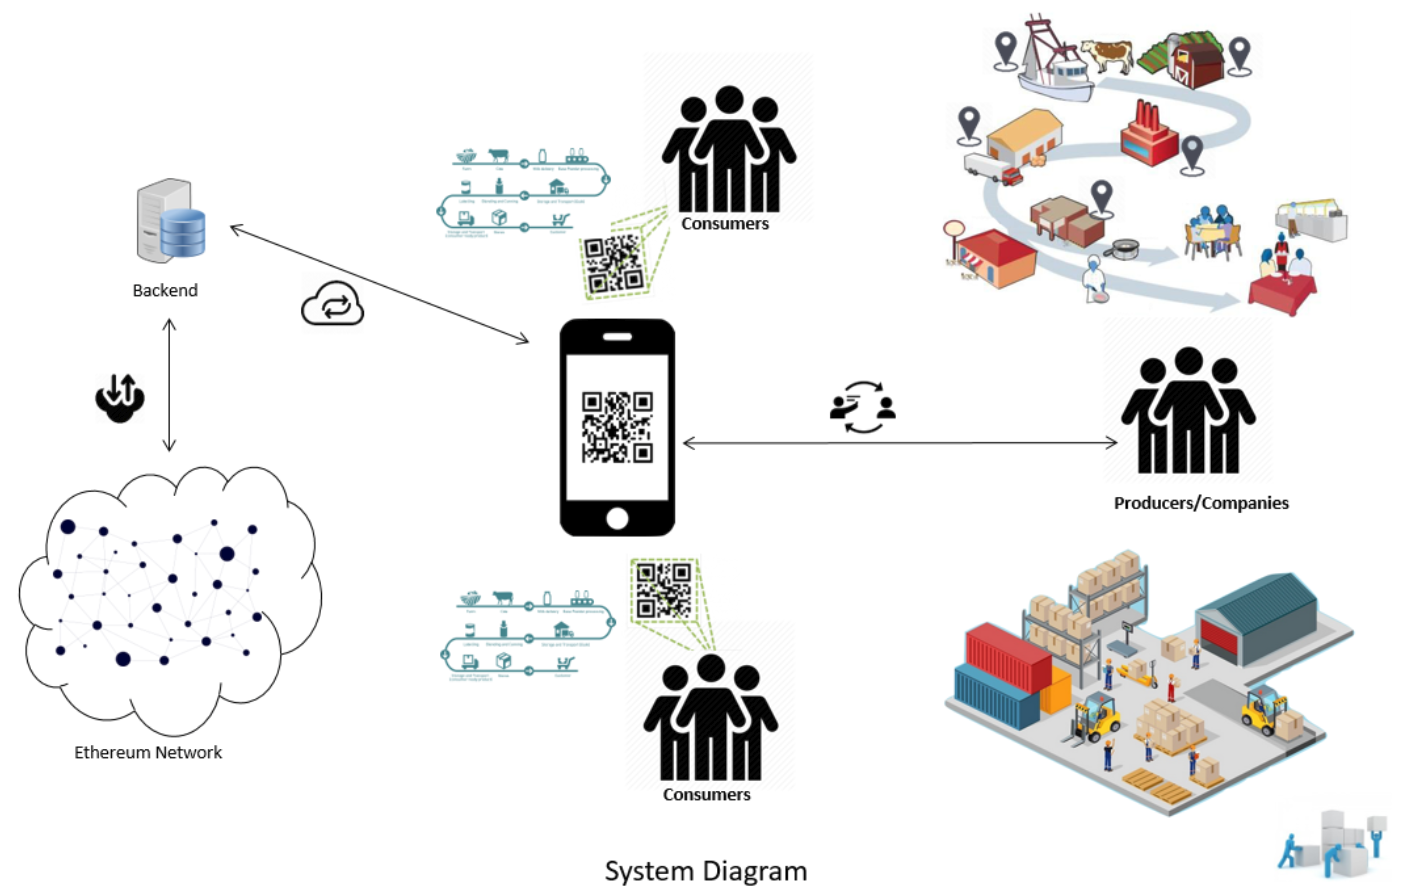
\includegraphics[width=\linewidth]{figures/system_diagram.png}
\caption{System Design Diagram \cite{atif_is}}
\label{fig:system_diagram}
\end{figure}

Figure \ref{fig:use_case_digram} shows the use-case diagram of the mobile application. The purpose of the use-case diagram is to show the interactions between the elements of the system.



\begin{figure}[ht]
\centering
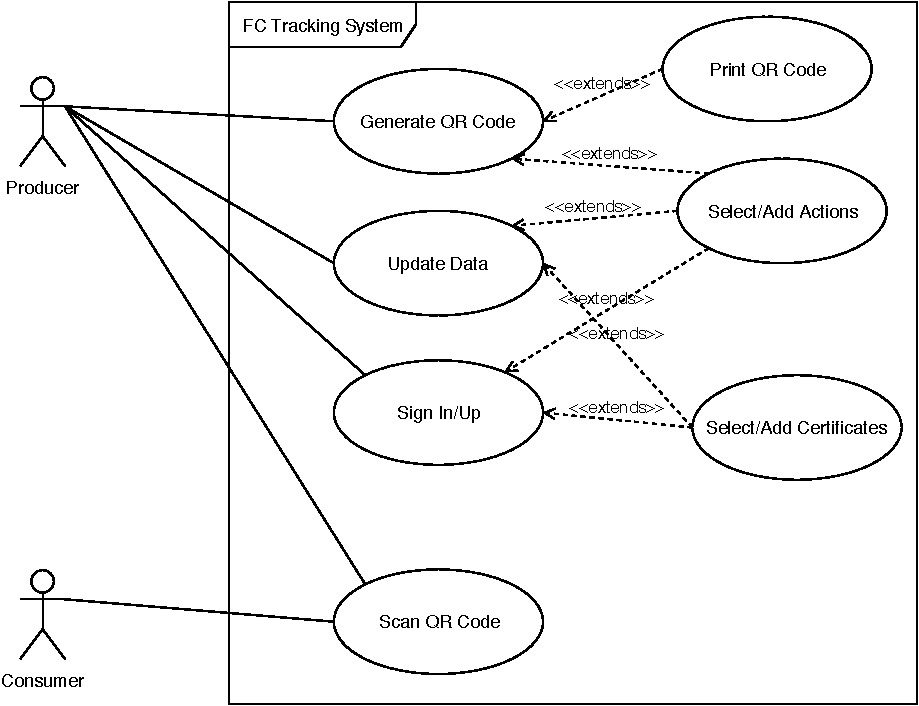
\includegraphics[width=0.7\columnwidth]{figures/use-case-diagram.pdf}
\caption{Use Case Diagram}
\label{fig:use_case_digram}
\end{figure}

 The given use case diagram can be breakdown into four main components: 
 
 \begin{enumerate}
     \item \textbf{System:} The application developed. In this case it represents the food chain tracking mobile application. It is a rectangle encompassing the use-cases and relationships. All components within this rectangle are the part of the system.
     
     \item \textbf{Actors:} Represent the external entities that use the functionalities provided by the system. In our case, the actors are the producers and consumers. 
     
     \item \textbf{Use-Cases:} The oval shaped elements representing the functionalities provided by the system, and used by the actors.
     
     \item \textbf{Relationships:} There are several types of relations.
        \begin{itemize}
            \item \textbf{Association:} Represented as a solid arrow. In this case there are the associations between the system and users, and consumers. Producer can generate QR code, sign in/up and update its data. On the other side, consumers can only scan products/QR codes and show the product's data. 
            \item \textbf{Extend:} Represented as a doted arrow, describes the use case that is extended by some additional functionalities. In this case, generating a QR code can be extended by the functionality that prints that newly generated QR code. 
        \end{itemize}
 \end{enumerate}
 
 \subsubsection{Container Diagram}

Figure \ref{fig:container-diagram} shows the container diagram. Essentially, every application represents one container that is runnable/deployable unit that process, stores or serves data. In that way, the benefits of using the micro-service architecture are lavereged. It represents the high-level view of the system architecture and how the responsibilities are distributed across containers. It also shows the major technology choices and how the containers communicate between each other.

The next part shortly explains each of the components.

\begin{description}
    \item[Database] 
    Food Chain Tracking System stores all its data in SQL database. All kind of SQL-like databases suported by Hibernate can be used to store the data.
    
    \item[RESTFul Web Service]
    Backend application exposing RESTFul APIs that other application can call.
    
    \item[Ethereum Node]
    In order to call the smart contract and validate product tag's hash, the backend applicaton calls the Ethereum node which can call the smart contract and validate the given hash value. The backend can easily switch to use a remote Ethereum node if e.g. the machine that the machine runs on doesn't have enough resources to run a node. 
    
    \item[Web Application]
    Application used by consumers. It is build as a sinlge-page web application and its production build is served by Nginx web server.
    
    \item[Reverse Proxy]
    Used in order to hide the internal structure of the system and increase the overall security. It exposes the server's and backend's APIs under the same origin. 
    
    \item[Android Appication]
    Used by producers that can create and validate product tags. It can also be used by consumers for checking the validity and details of product tags.
    
    \item[React Native Application]
    Mobile application build with React Native framework that provides the same look and feel on both Android and iOS platforms.It can also be used by both producers and consumers and it is intended to provide the same functionalities as aforementioned Andoroid application.
    
    \item[Ethereum Network]
    A distributed-computing platform and operating system featuring smart contract functionality. It runs the smart contract written for this platform and executes the transactions against the contract. 
\end{description}

\begin{figure}[ht]
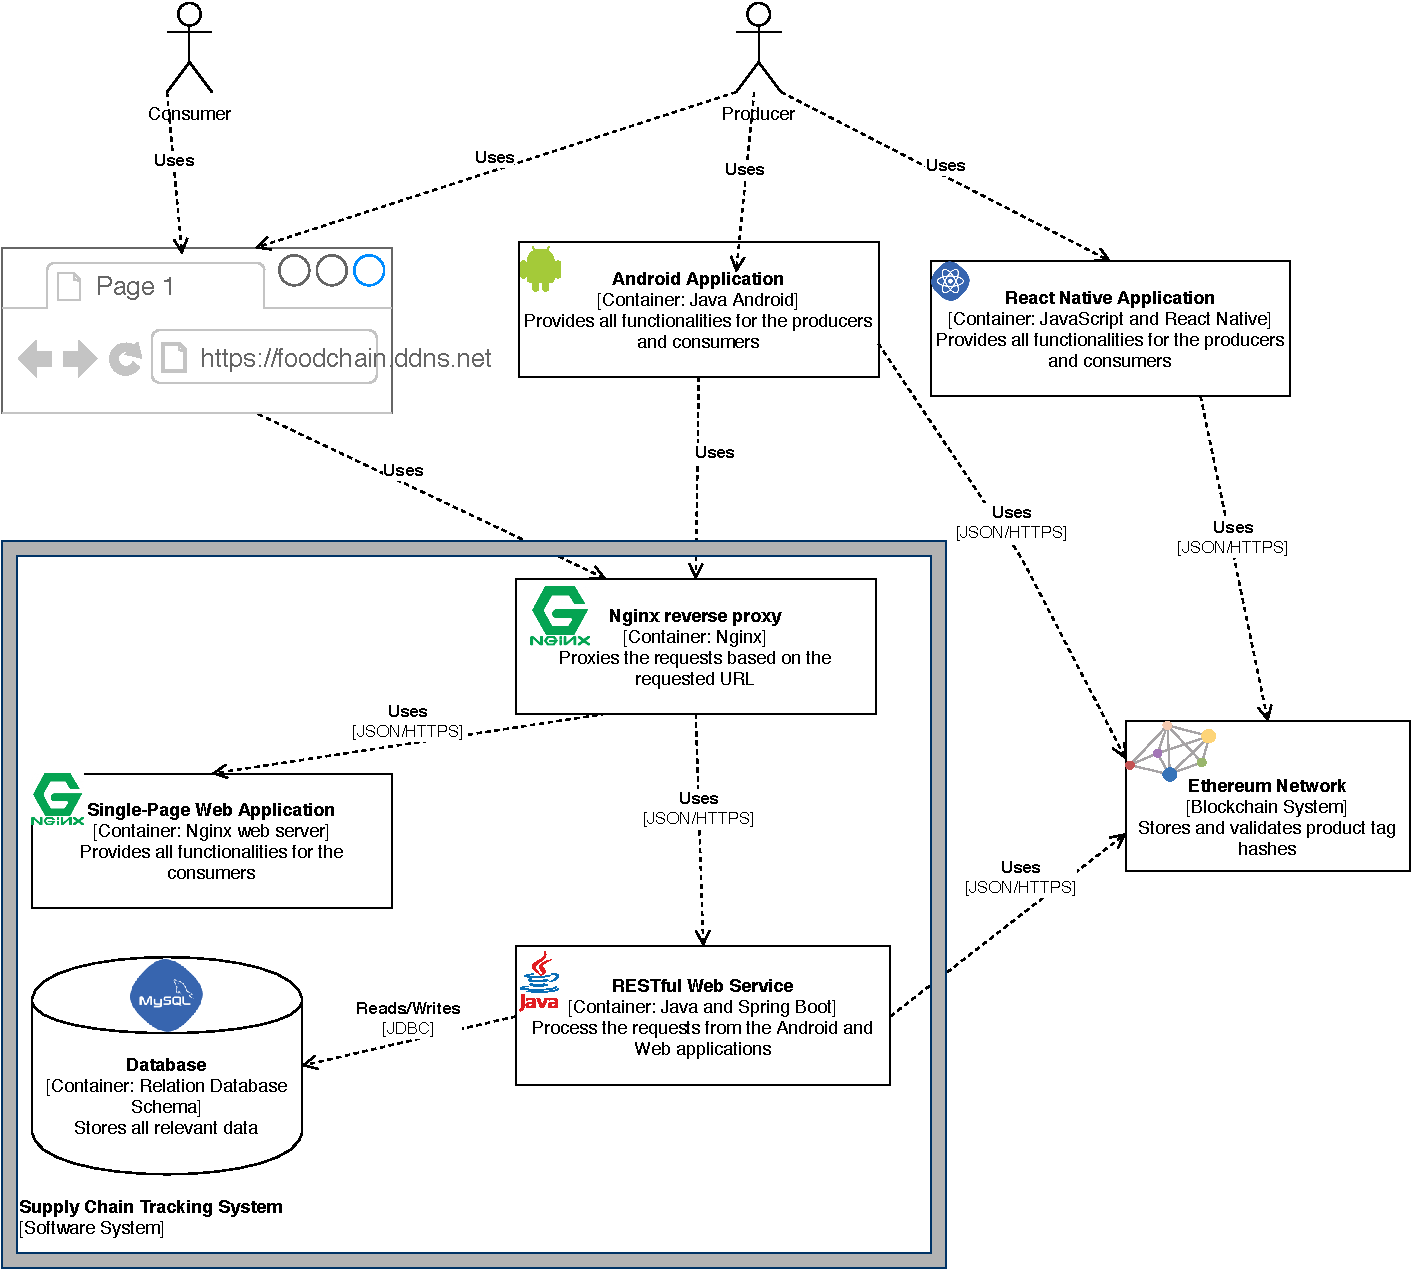
\includegraphics[width=\linewidth]{figures/container-diagram.pdf}
\caption{Container Diagram for Food Chain Tracking System.}
\label{fig:container-diagram}
\end{figure}

This overview of the whole ecosystem is given in order to show the role of the Application being built. In the next section the implementation details will be explained. 


\section{Implementation}

This section covers the implementation details for the Food Chain Mobile Application. 
The main goal of this mobile application is to bring the supply chain platform to the producers and consumers using the iOS platform. Therefore, the requirement was to build the mobile application that can run on the iOS platform. There were several possible technologies/frameworks available for building an iOS application and in the end, the React Native framework was used. This section will explain the React Native internals, reasons why the React Native was used, and also the implementation details will be given. 

\subsection{React Native}

React Native is a JavaScript framework for writing real, natively rendering mobile applications for iOS and Android. It is based on React \cite{react}, Facebook's JavaScript library for building user interfaces, but instead of targeting the browser, it targets mobile platforms. React Native currently supports both iOS and Android, and has the potential to expand to future platforms as well \cite{rn_oreilly}.

The fact that by writing Java Script code and running it natively on both Android and iOS platforms brings clear benefits. Only one code base should be maintained while utilizing well established frameworks/tools such as React \cite{react}, Redux\cite{redux}, Material-UI \cite{material_ui} etc. 

As mentioned, React Native provides almost native performances. The reason is because the code written in Java Script gets compiled natively to the target platforms where currently Android and iOS are supported. Also, the support for a few other platforms are under development \cite{rn_platform_development}. Figure \ref{fig:rn_compiling} illustrates the flow of the compiling process. 

\begin{figure}[ht]
\centering
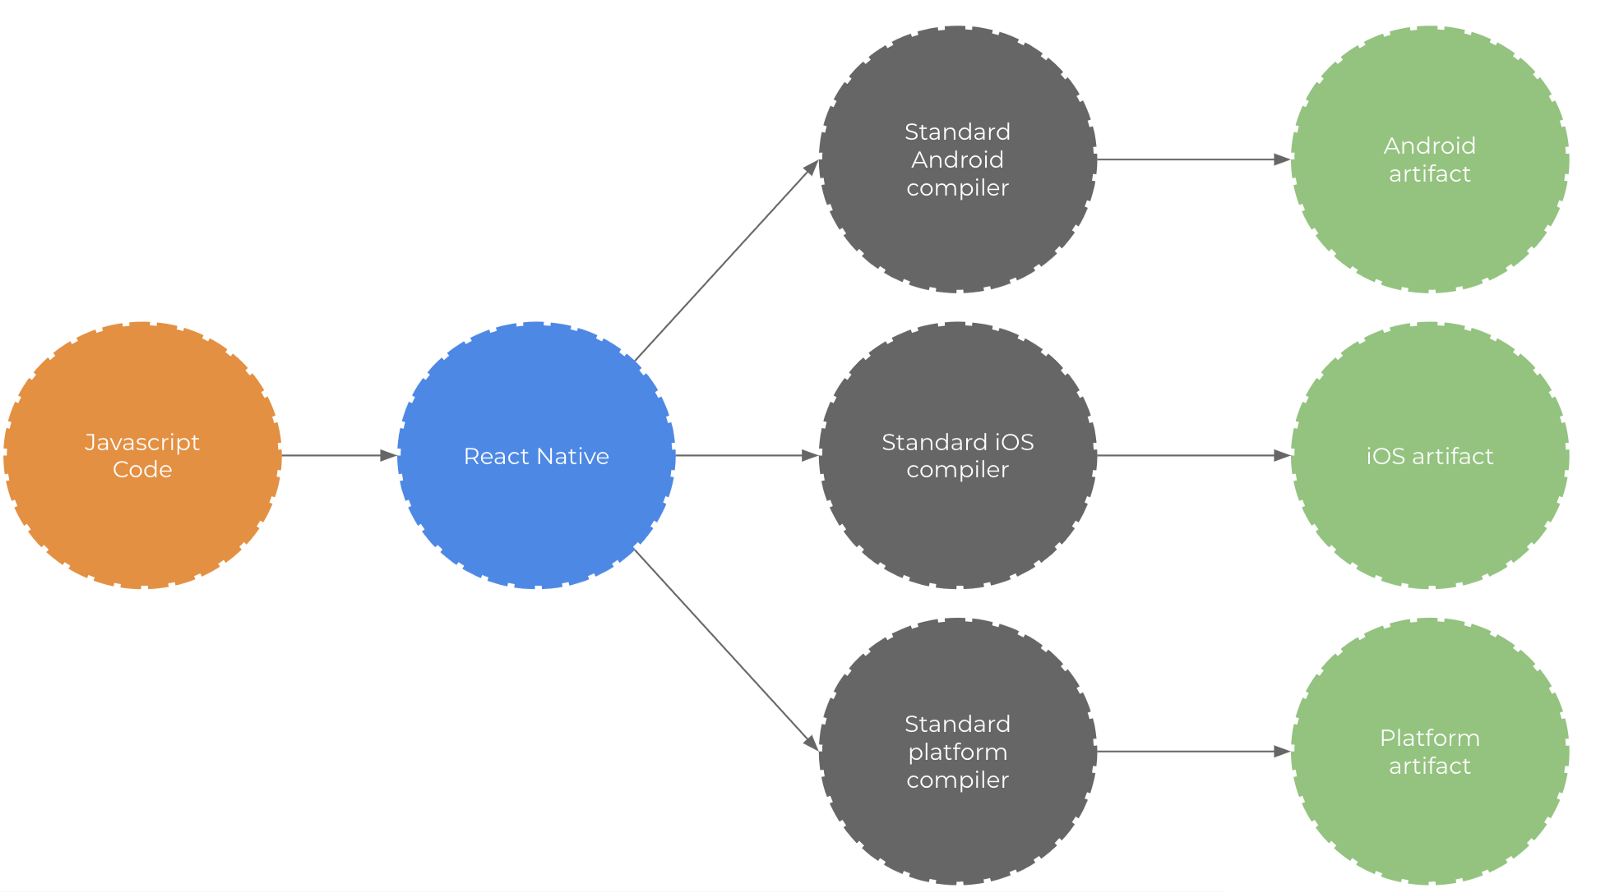
\includegraphics[width=0.7\columnwidth]{figures/rn-compiler.png}
\caption{React Native compiling flow \cite{rn_bridge_article}}
\label{fig:rn_compiling}
\end{figure}

The heart of the React Native architecture is the bridge that allows the communication between JavaScript and a native/target platform. The bridge provides bidirectional and asynchronous communication between these two different technologies. The figure \ref{fig:rn_bridge} illustrates the communication between two different technologies using the bridge. 


\begin{figure}[ht]
\centering
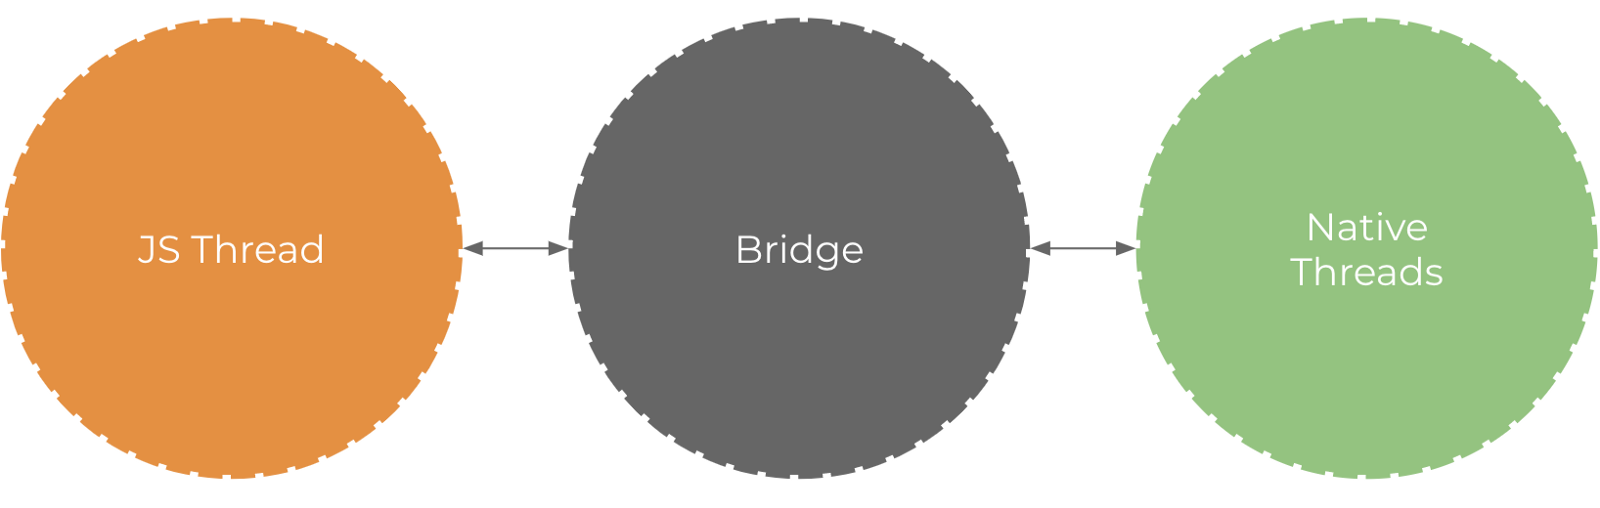
\includegraphics[width=0.7\columnwidth]{figures/rn-bridge.png}
\caption{Bridge sitting between JavaScript and Native Threads \cite{rn_bridge_article}}
\label{fig:rn_bridge}
\end{figure}

\subsection{State Management} 

Managing application state is a crucial component in any software development process. React itself provides some useful methods for setting component's state using \texttt{setState()} and adding a 'local state' to a class. The method \texttt{setState()} will set the state in the corresponding class, which means that the changed state will be accessible just inside that class and its children classes and components. Managing states just with React is possible but very ineffective due to growing complexity and performance issues, especially as the application grows. 

Redux \cite{redux} is a library that helps to manage application state in consistent and predictable manner. The Redux Store is basically the single source of true for the application and it can be changed only with pure functions \cite{pure-function}. The React component can connect to the Redux store by using the \texttt{react-redux} library\cite{react-redux}. That allow the components to subscribe to the Store changes, and also trigger the update on the Store.

The figure \ref{fig:redux-flow} shows the Redux flow in React applications. It is important to mention that when making the asynchronous calls, the additional middleware has to be used that will update the Redux Store on the call completion. In this application, for that purpose Redux Thunk \cite{redux-thunk} was utilized.  

\begin{figure}[ht]
\centering
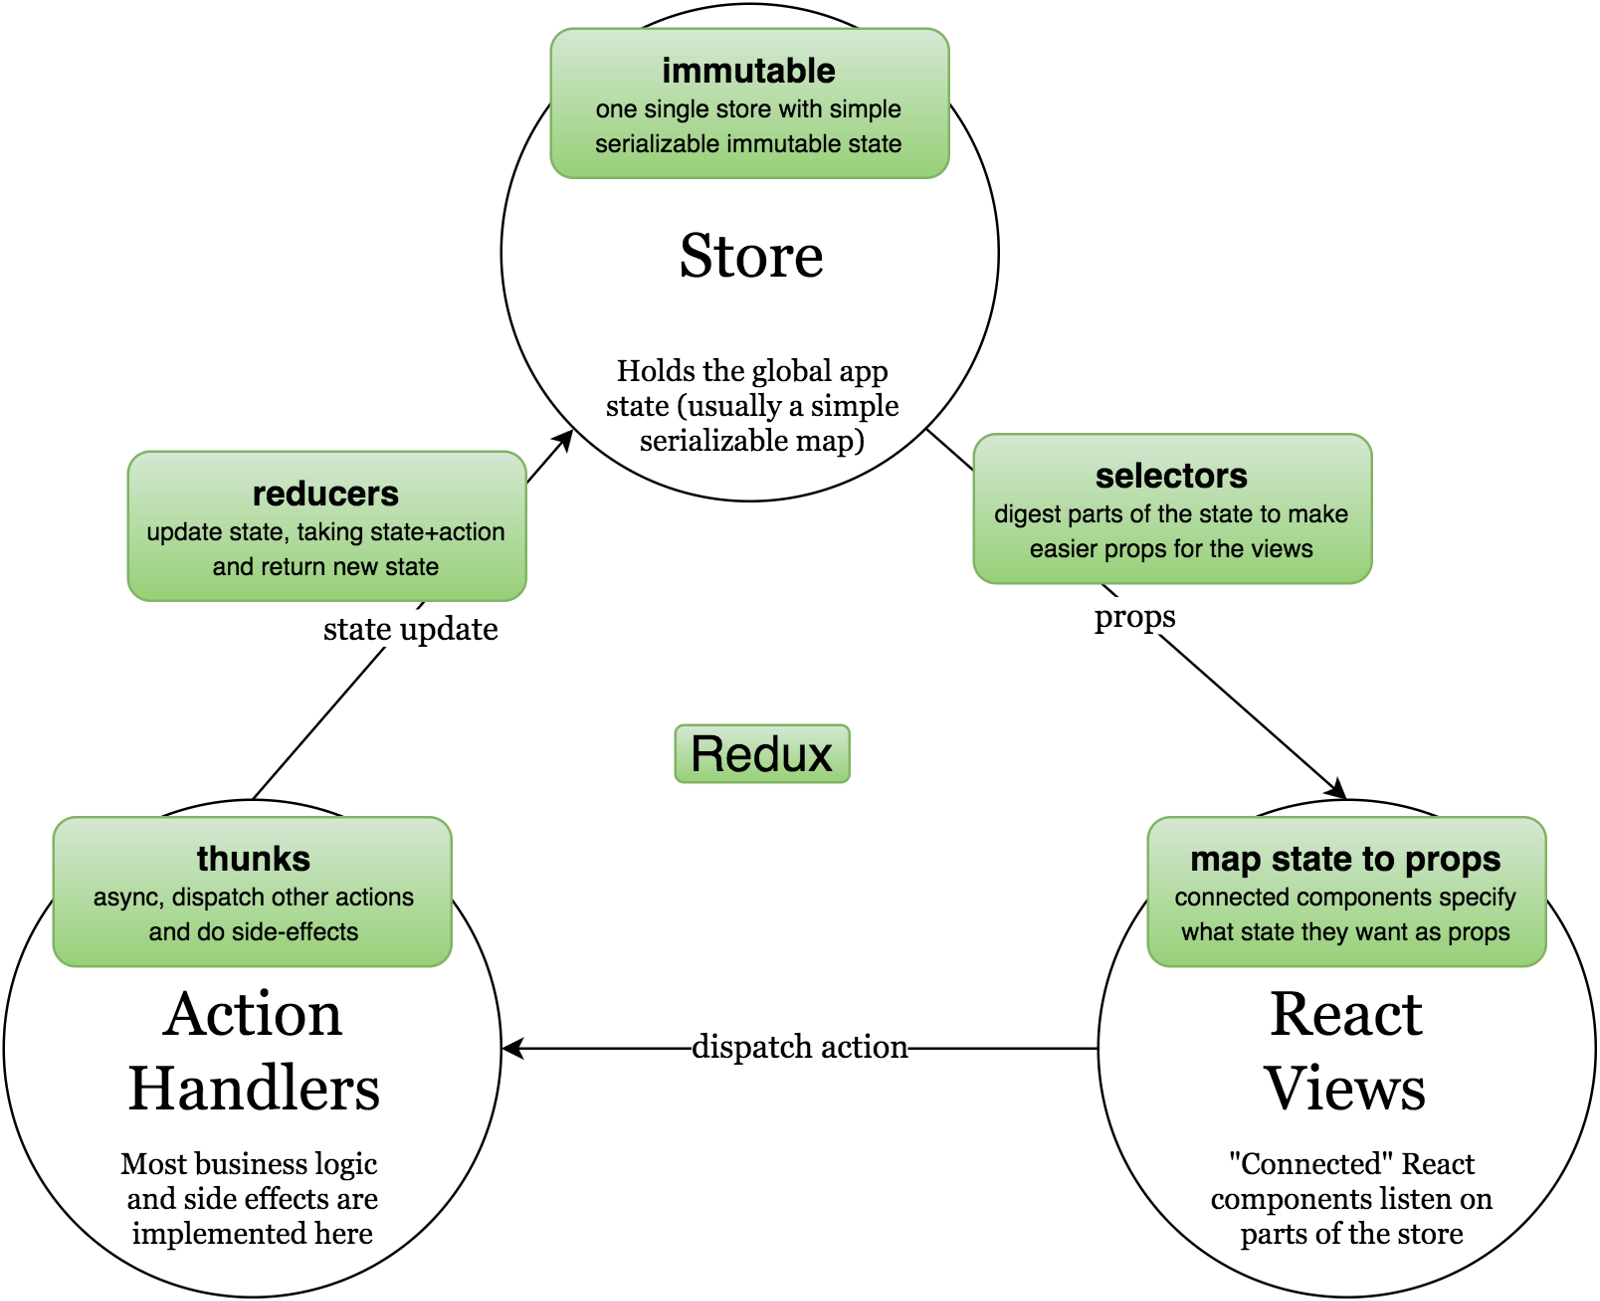
\includegraphics[width=0.7\columnwidth]{figures/redux-flow.png}
\caption{Redux Flow\cite{redux-flow}}
\label{fig:redux-flow}
\end{figure}

Section \ref{sec:milti-language} explains how the Redux library was utilized to implement the multi-language support.

\subsection{Multi-Language Support}\label{sec:milti-language}

As the global application state is handled with Redux \cite{redux}, the multi-language support is implemented with the same library. The language can be changed from the home screen drawer. Currently, German, English, French and Italian are implemented. Figure \ref{fig:app-drawer} shows the open drawer where the buttons for the implemented languages are shown. The button for the current language is in blue color. By changing the language, the Redux Store gets updated which triggers the text to change in the whole application. This allows the managing of all the translations of the application from one central place. All components that have to display some of the translations, just have to subscribe to the global Store using the aforementioned \texttt{react-redux} library, and select the key of the corresponding text.

Figure \ref{fig:app-homescreen-german} shows the home screen in German language while \ref{fig:app-homescreen} shows the same screen in English translation. 

\begin{figure}[!h]
	\centering
	\begin{minipage}[t]{4cm}
		\centering
		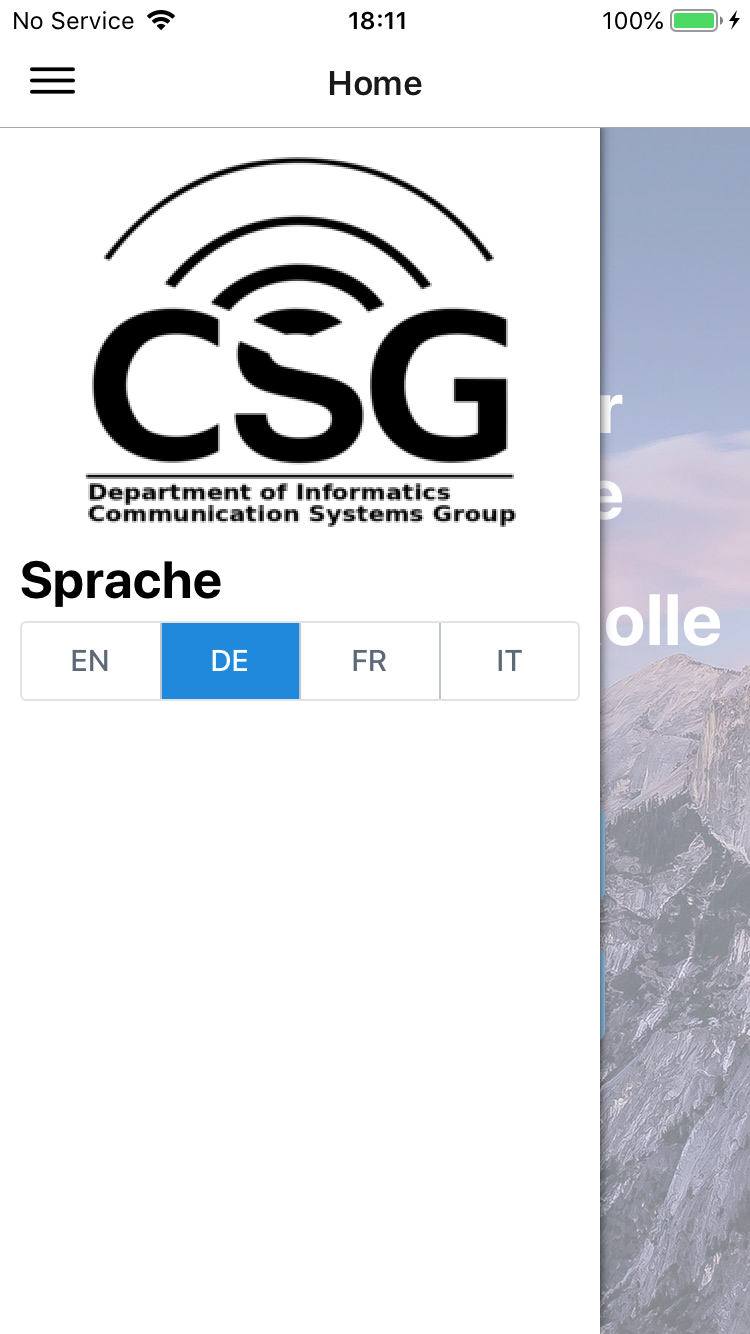
\includegraphics[width=5.5cm, height=10cm]{figures/app-2.PNG}
		\caption{Home screen drawer}
		\label{fig:app-drawer}
	\end{minipage}
	\hspace{3cm}
	\begin{minipage}[t]{4cm}
		\centering
		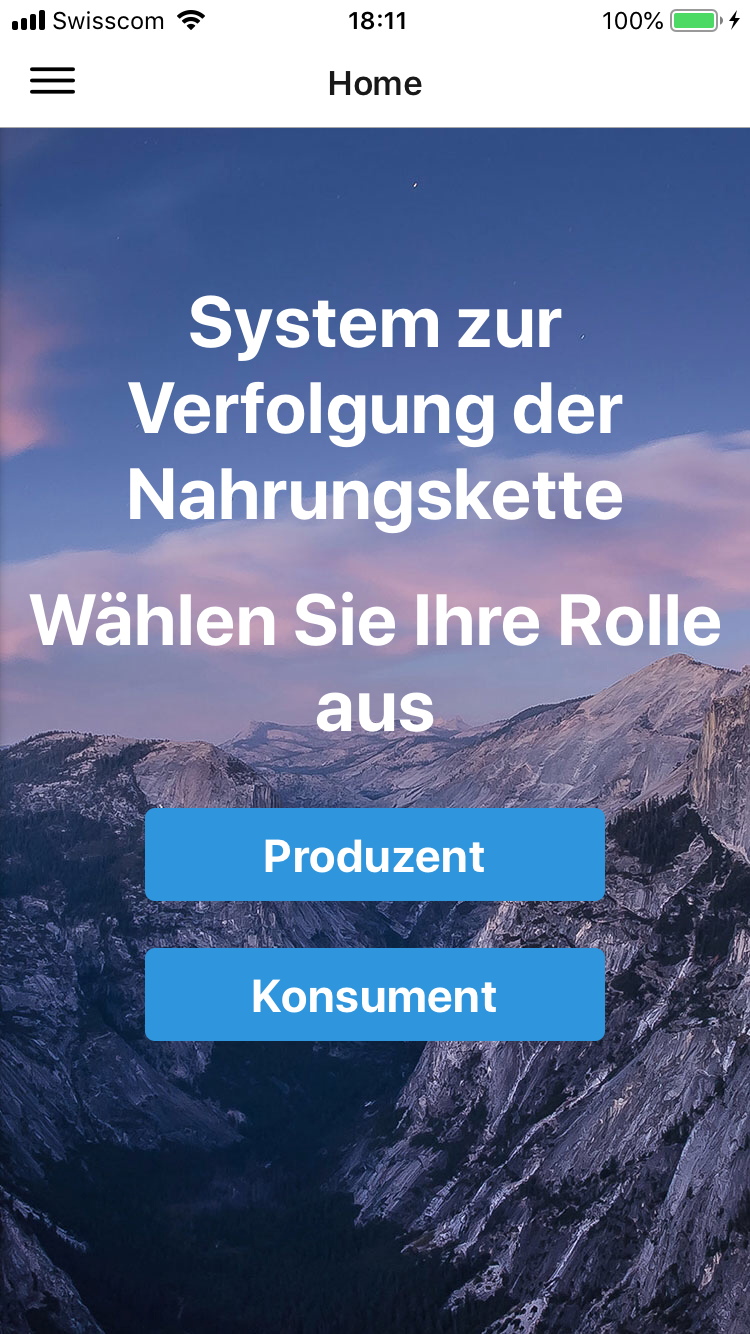
\includegraphics[width=5.5cm, height=10cm]{figures/app-4.PNG}
		\caption{Home screen - German translation}
		\label{fig:app-homescreen-german}
	\end{minipage}
\end{figure}


\section{Application Modes}

As mentioned, the Food Chain Mobile Application provides the functionalities for both producers and consumers. 

\subsection{Producer Mode}

The producer mode of the application provides a wide set of functionalities that help the producers to successfully use the Food Chan Tracking system. As shown in \ref{fig:use_case_digram}, producers can login, register, add or create actions and certificates, generate QR code, see the QR codes they have generated, update their data. 
Producer's authentication screen can be entered by pressing the Producer button from the home screen. 

\begin{figure}[!h]
	\centering
	\begin{minipage}[t]{4cm}
		\centering
		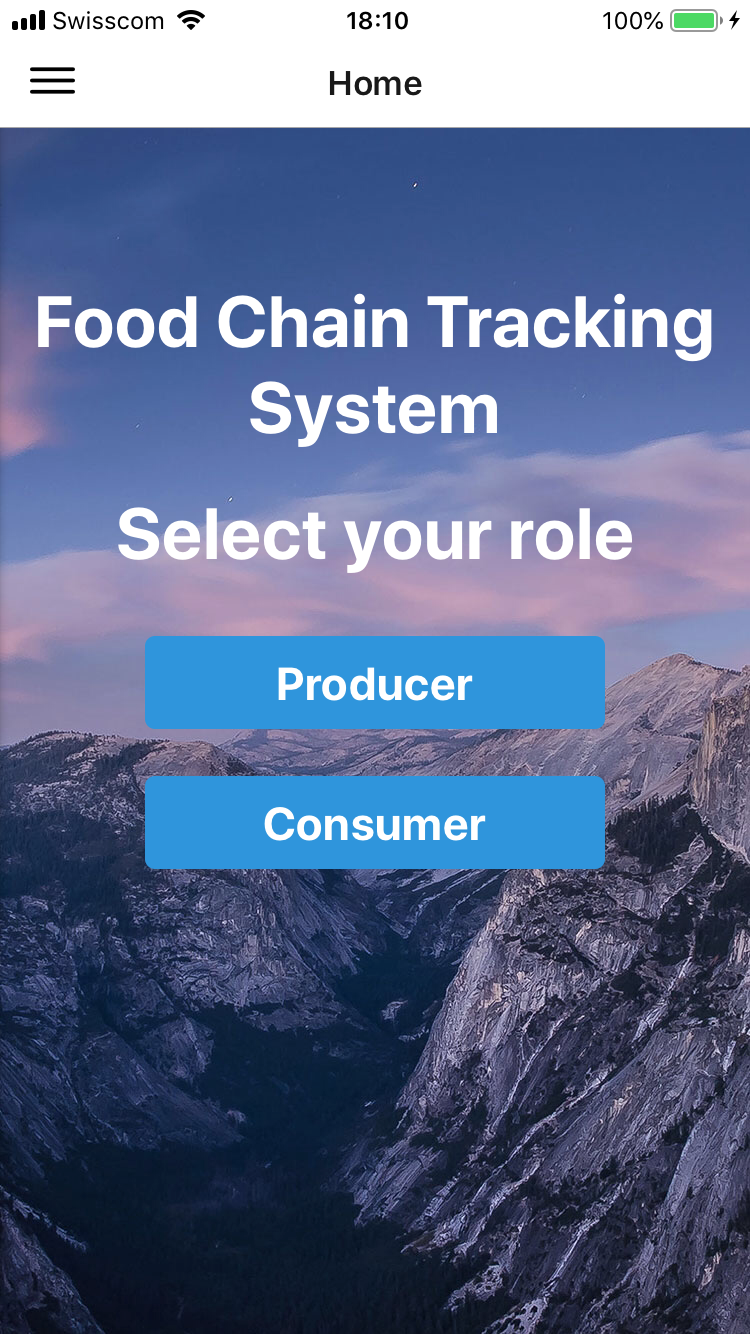
\includegraphics[width=5.5cm, height=10cm]{figures/app-1.PNG}
		\caption{Home screen}
		\label{fig:app-homescreen}
	\end{minipage}
	\hspace{3cm}
	\begin{minipage}[t]{4cm}
		\centering
		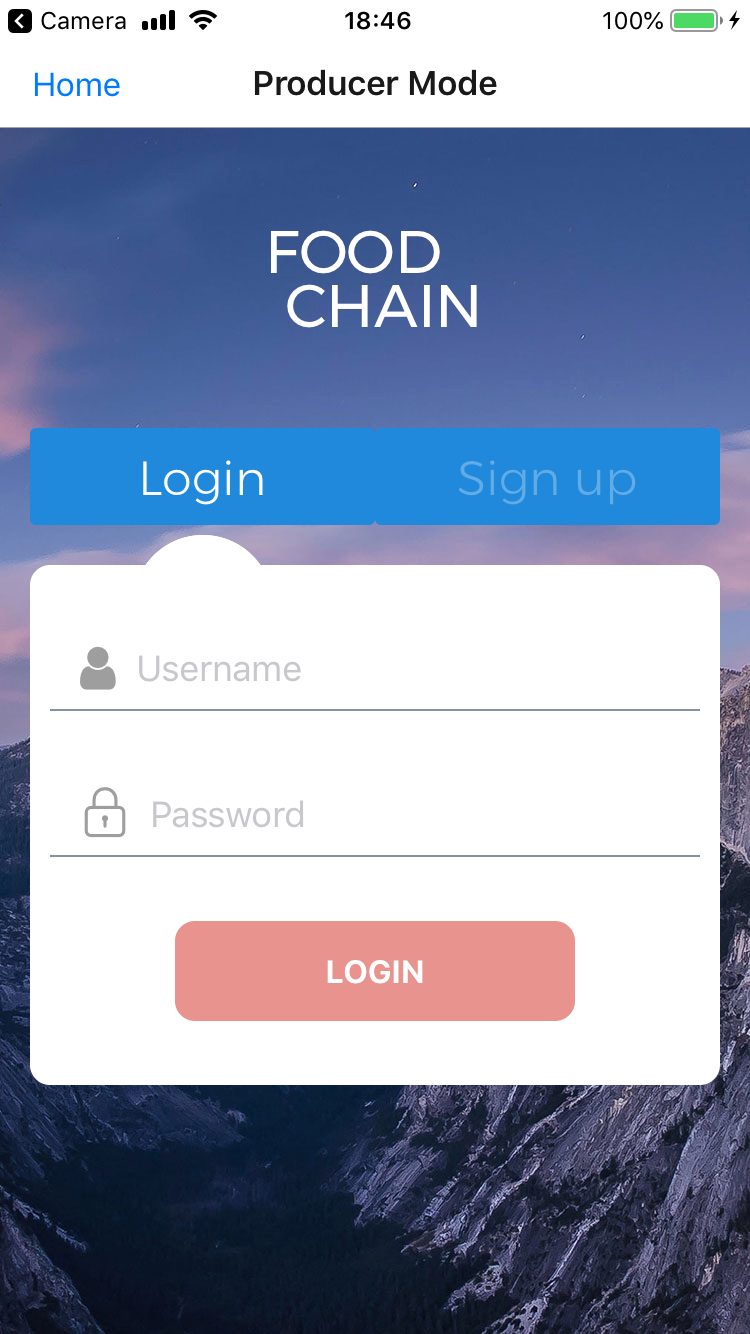
\includegraphics[width=5.5cm, height=10cm]{figures/app-3.PNG}
		\caption{Producer Login Screen}
		\label{fig:app-login-screen}
	\end{minipage}
\end{figure}


\begin{figure}[!h]
	\centering
	\begin{minipage}[t]{4cm}
		\centering
		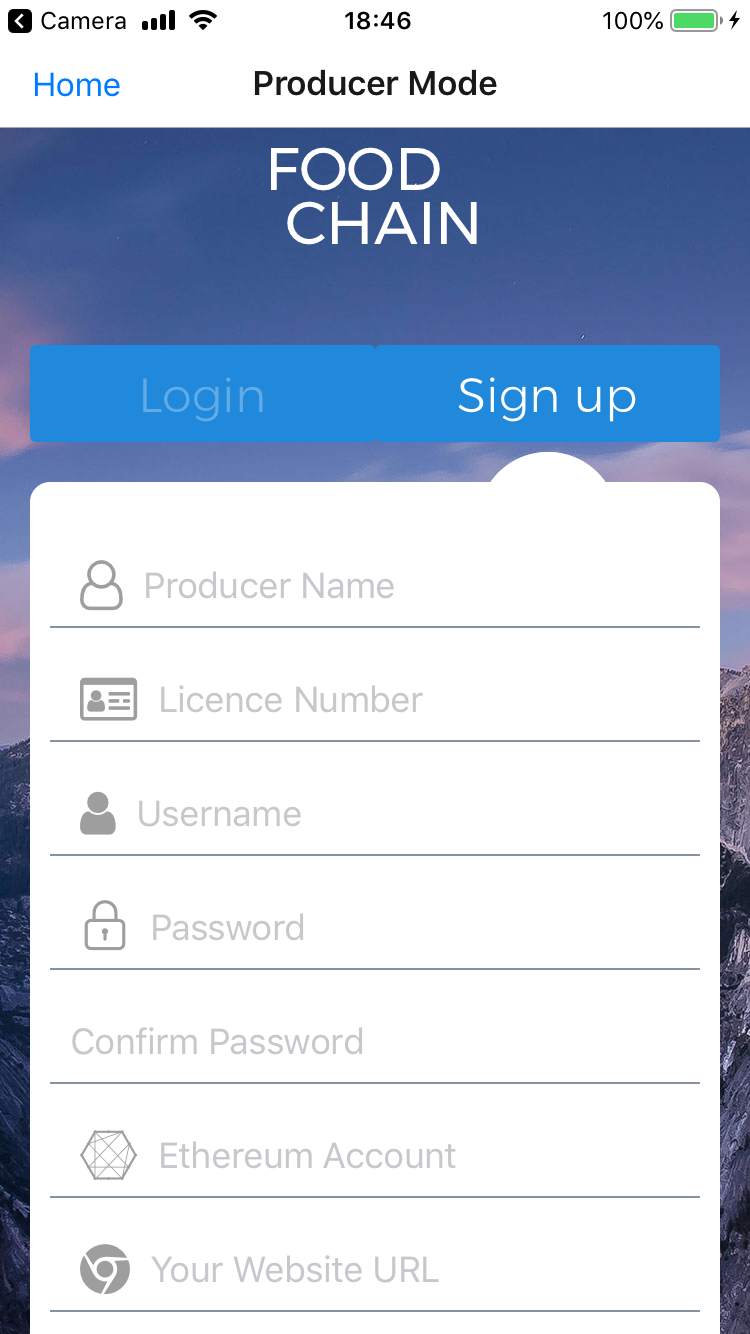
\includegraphics[width=5.5cm, height=10cm]{figures/app-5.PNG}
		\caption{Producer Sign-up Screen}
		\label{fig:app-sign-up-screen}
	\end{minipage}
	\hspace{3cm}
	\begin{minipage}[t]{4cm}
		\centering
		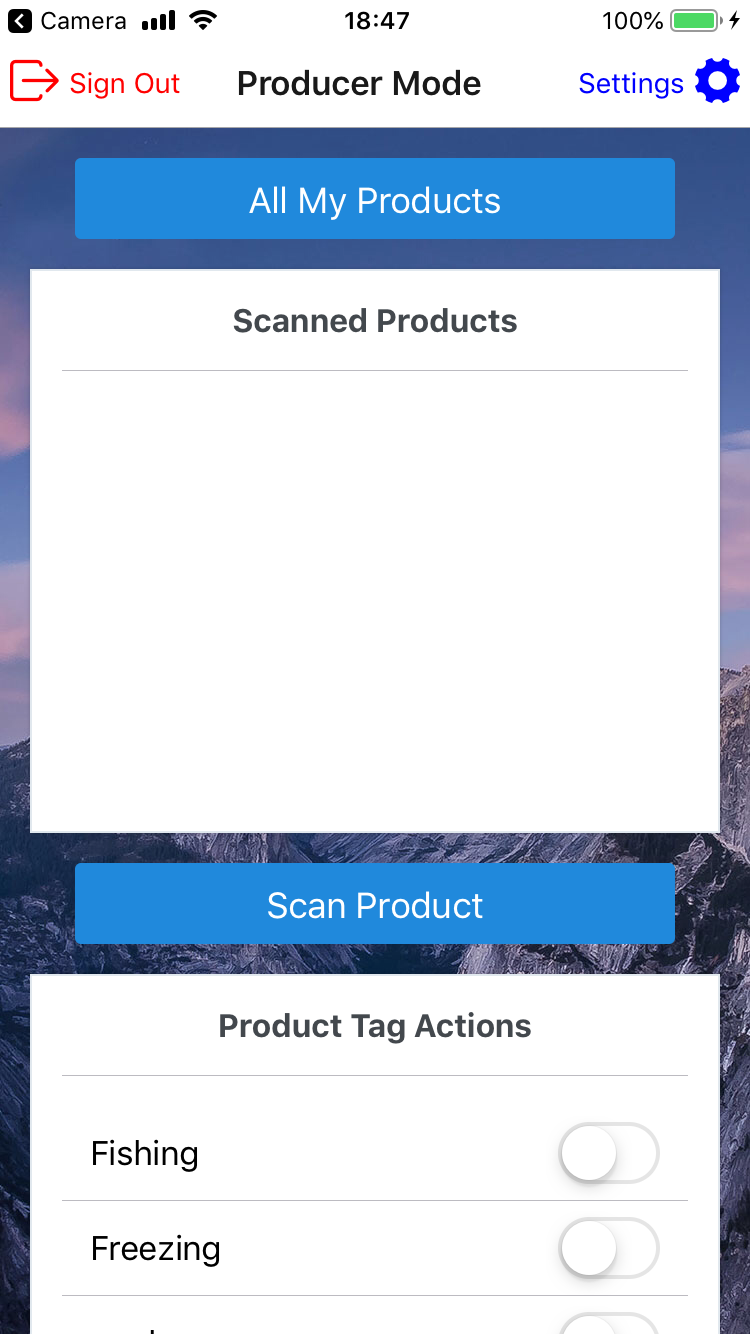
\includegraphics[width=5.5cm, height=10cm]{figures/app-6.PNG}
		\caption{Producer Home Screen}
		\label{fig:app-producer-home-screen}
	\end{minipage}
\end{figure}


\begin{figure}[!h]
	\centering
	\begin{minipage}[t]{4cm}
		\centering
		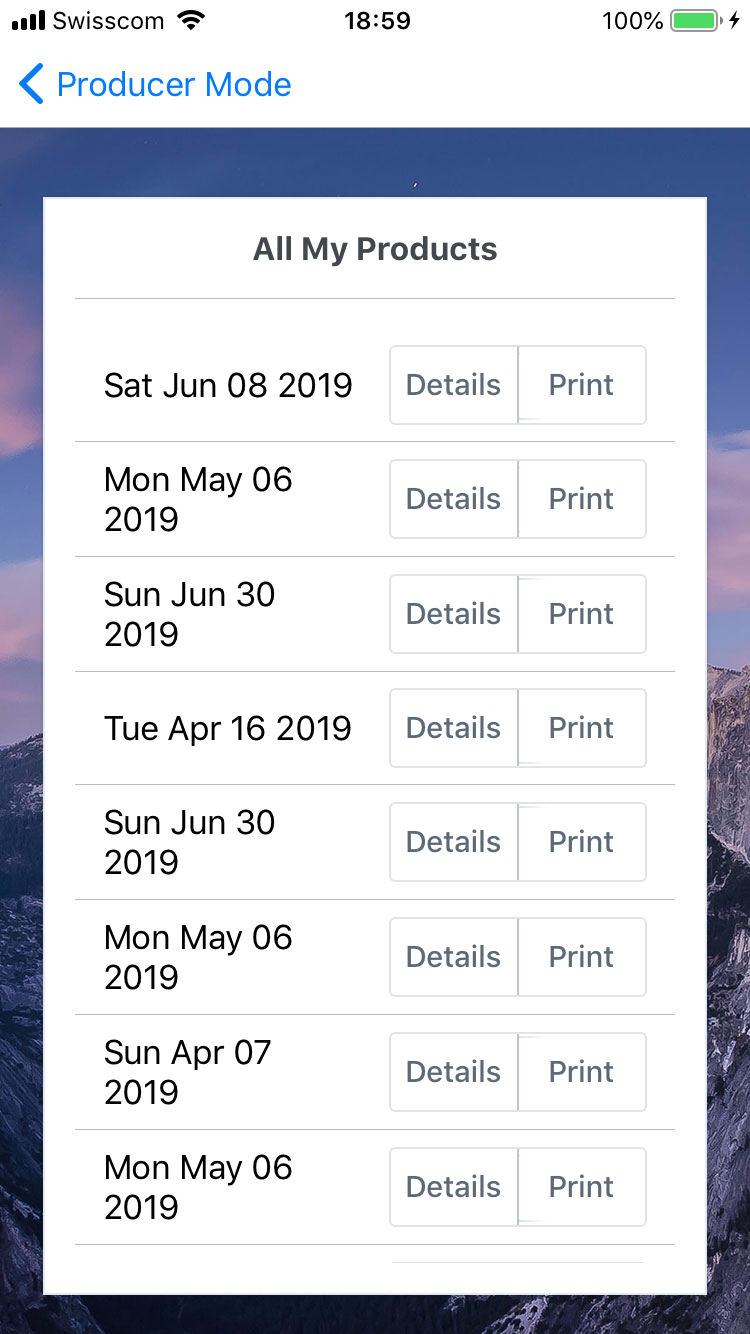
\includegraphics[width=5.5cm, height=10cm]{figures/app-7.PNG}
		\caption{Producer's Product History Screen}
		\label{fig:app-producer-product-history-screen}
	\end{minipage}
	\hspace{3cm}
	\begin{minipage}[t]{4cm}
		\centering
		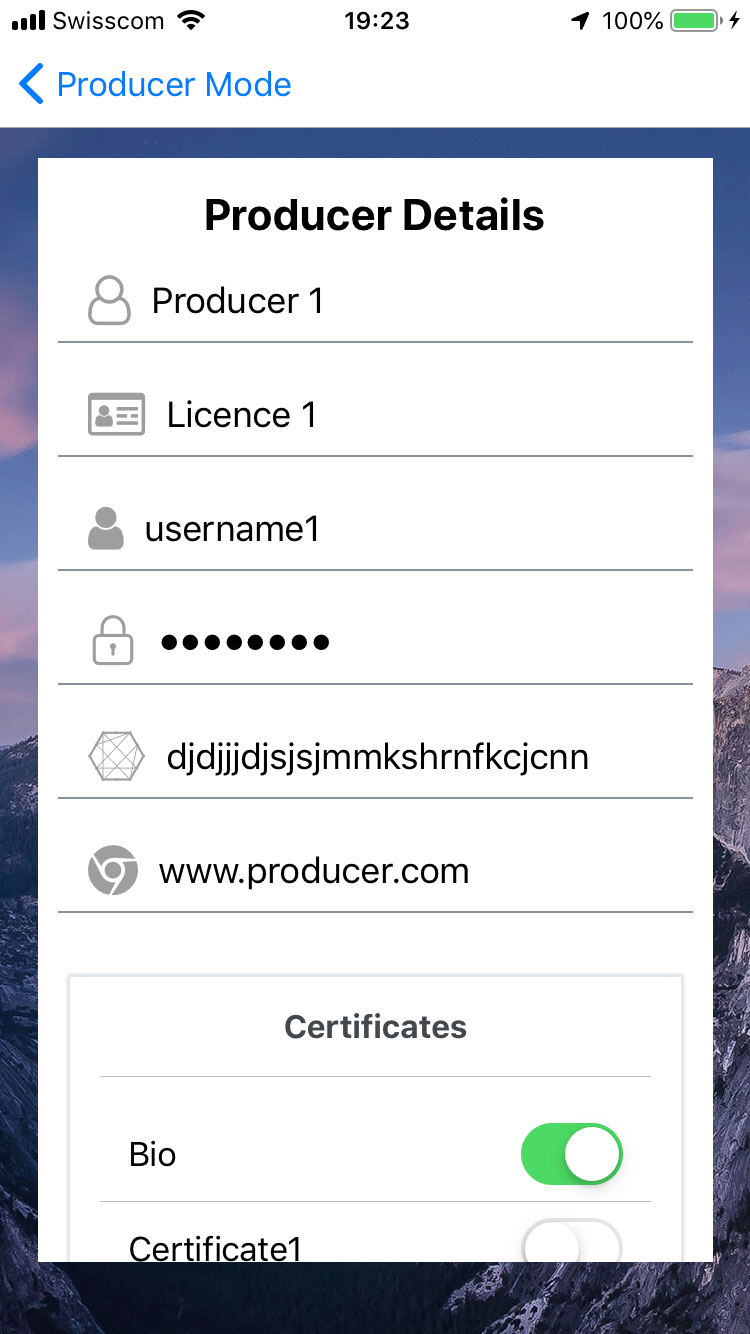
\includegraphics[width=5.5cm, height=10cm]{figures/app-8.PNG}
		\caption{Producer Update Screen}
		\label{fig:app-producer-update-screen}
	\end{minipage}
\end{figure}


\subsection{Consumer Mode}

\chapter{Evaluation and System Analysis}

\chapter{Summary and Future Considerations}


\begin{thebibliography}{99}



\end{thebibliography}



% \printbibliography

\chapter*{Abbreviations}
\addcontentsline{toc}{chapter}{Abbreviations}
\markboth{ABBREVIATONS}{}



\abr{REST}{Representational State Transfer}
\abr{API}{Application Programming Interface}
\abr{SQL}{Structured Query Language}



\addcontentsline{toc}{chapter}{List of Figures}
\listoffigures
\addcontentsline{toc}{chapter}{List of Tables}
\listoftables

\appendix

\chapter{Installation Guidelines}


\end{document}
